% Copyright (c) 2017-2019  Zubax Robotics  <info@zubax.com>
%
% Distributed under BY-NC-ND (attribution required, non-commercial use only, no derivatives).
%

\documentclass{zubaxdoc}
\graphicspath{{document_templates/documentation_template_latex/}}
\title{Zubax Sadulli Datasheet}

\hbadness=10000

% To be removed when ready for publication
\usepackage{draftwatermark}
\SetWatermarkScale{1.2}
\SetWatermarkLightness{0.9}

\begin{document}
\frontmatter
\begin{titlepage}
\section*{Overview}
Zubax Sadulli is a tightly integrated unit that contains an electric motor with electronic speed controller (ESC). 
This sensorless propeller drive is an open hardware reference design for Mitochondrik module
\footnote{Refer to \url{https://zubax.com//products/mitochondrik} for more information}.
\section*{Features}

\begin{itemize}
    \item 550 W continuous power output.
    \item 4S - 8S wide power voltage range.
    \item 5v, 0.5 A BEC.
    \item High-efficiency sensorless FOC algorithms.
    \item Self-diagnostics and health status reporting.
    \item Built-in motor temperature sensor for enhanced \allowbreak{}self-diagnostics.
    \item Ready right out of the box. All parameters are tuned for high dynamic response and high-efficiency work.      
    \item Highly configurable. All parameters can be changed. The firmware can be upgraded by the user.     
    \item Regenerative braking and active freewheeling. 
    \item Solder-free design facilitates in-field maintenance.
    \item Low noise and high efficiency due to the sinusoidal motor currents and \allowbreak{}high-frequency PWM.
    \item Supported interfaces:
    \begin{itemize}
        \item UAVCAN\footnote{Refer to \url{https://uavcan.org/} for more information}.
        \item RCPWM (optional).
    \end{itemize}
    \item High quality assurance:
    \begin{itemize}
        \item Every manufactured unit undergoes a strict testing procedure.
        The testing log for each produced unit is available to the user via the website at
        \url{https://device.zubax.com/device_info}.
        \item Protection against unlicensed (counterfeit) production by means of a digital signature installed on 
        every manufactured unit.
     \end{itemize}
\end{itemize}

\section*{Applications}

\begin{itemize}
    \item Propeller drives for multirotor unmanned aerial vehicles.
    \item Pump and propeller drives for unmanned watercraft.
\end{itemize}
\centering
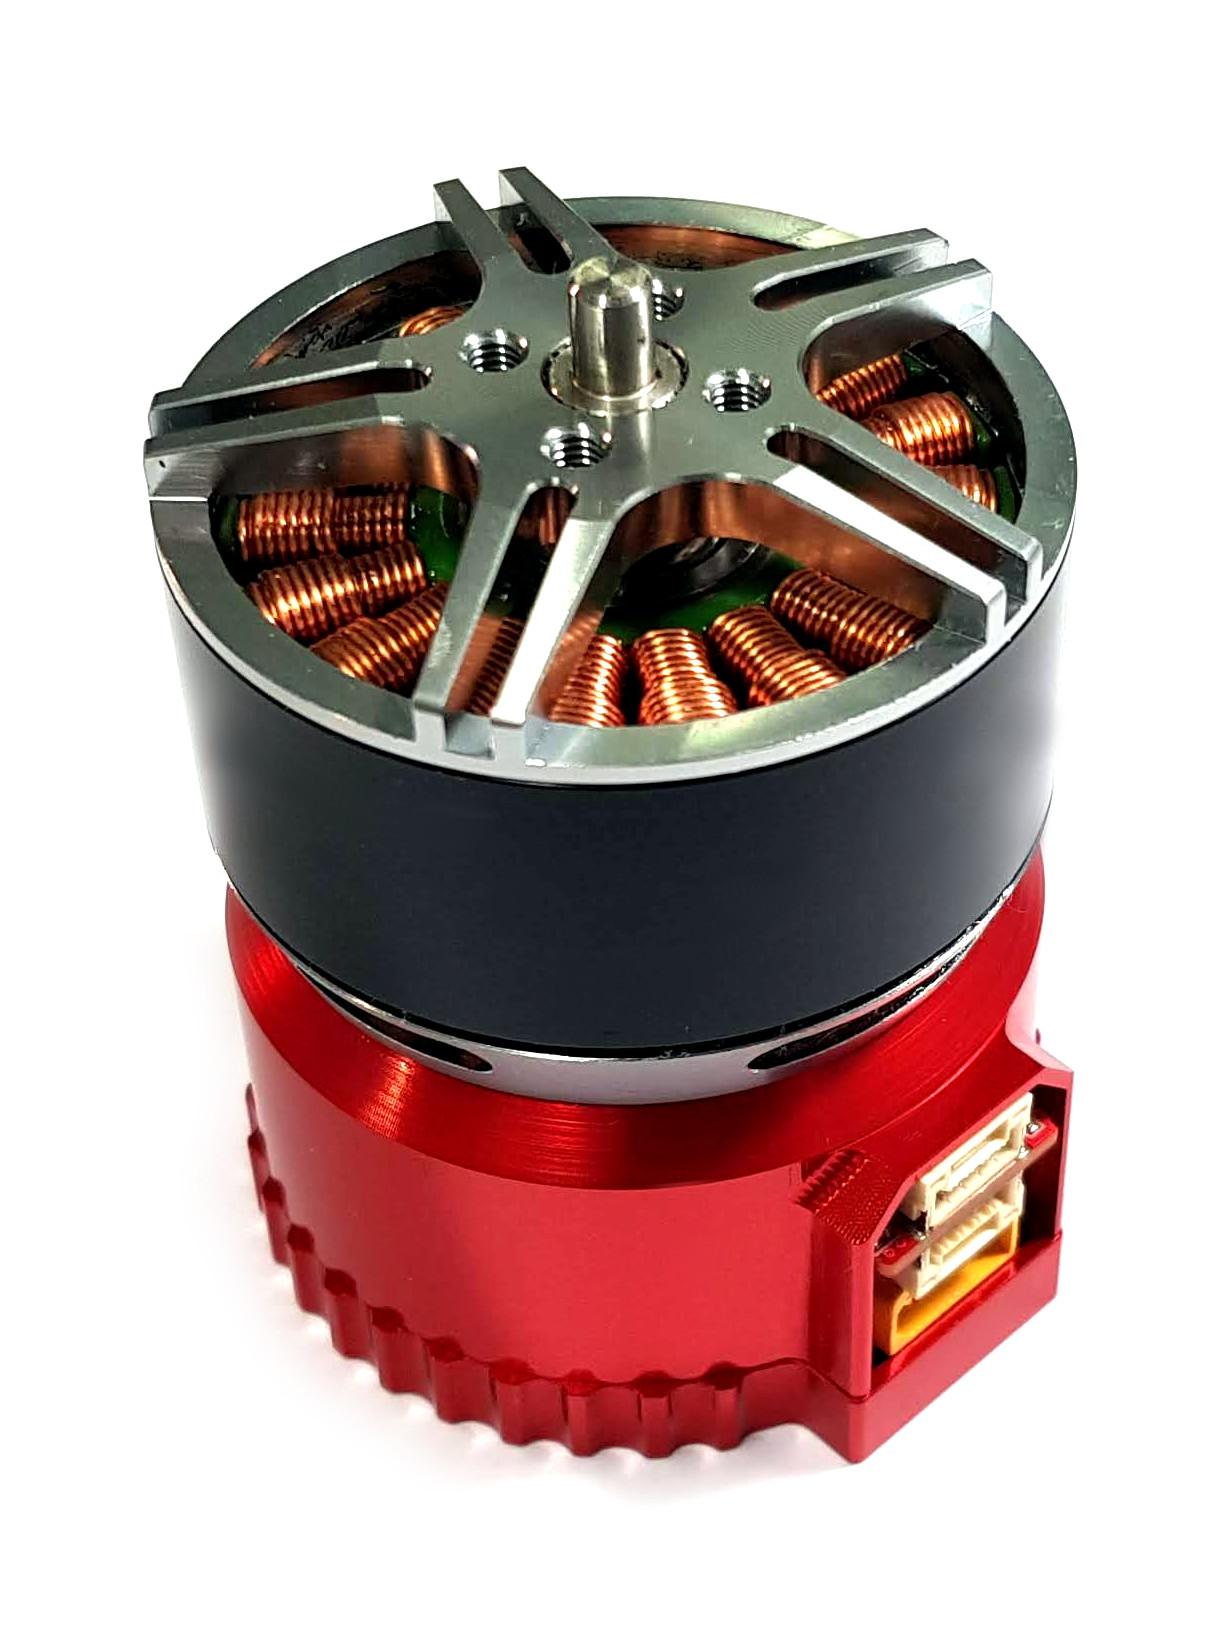
\includegraphics[width=0.42\textwidth]{sadulli-top}
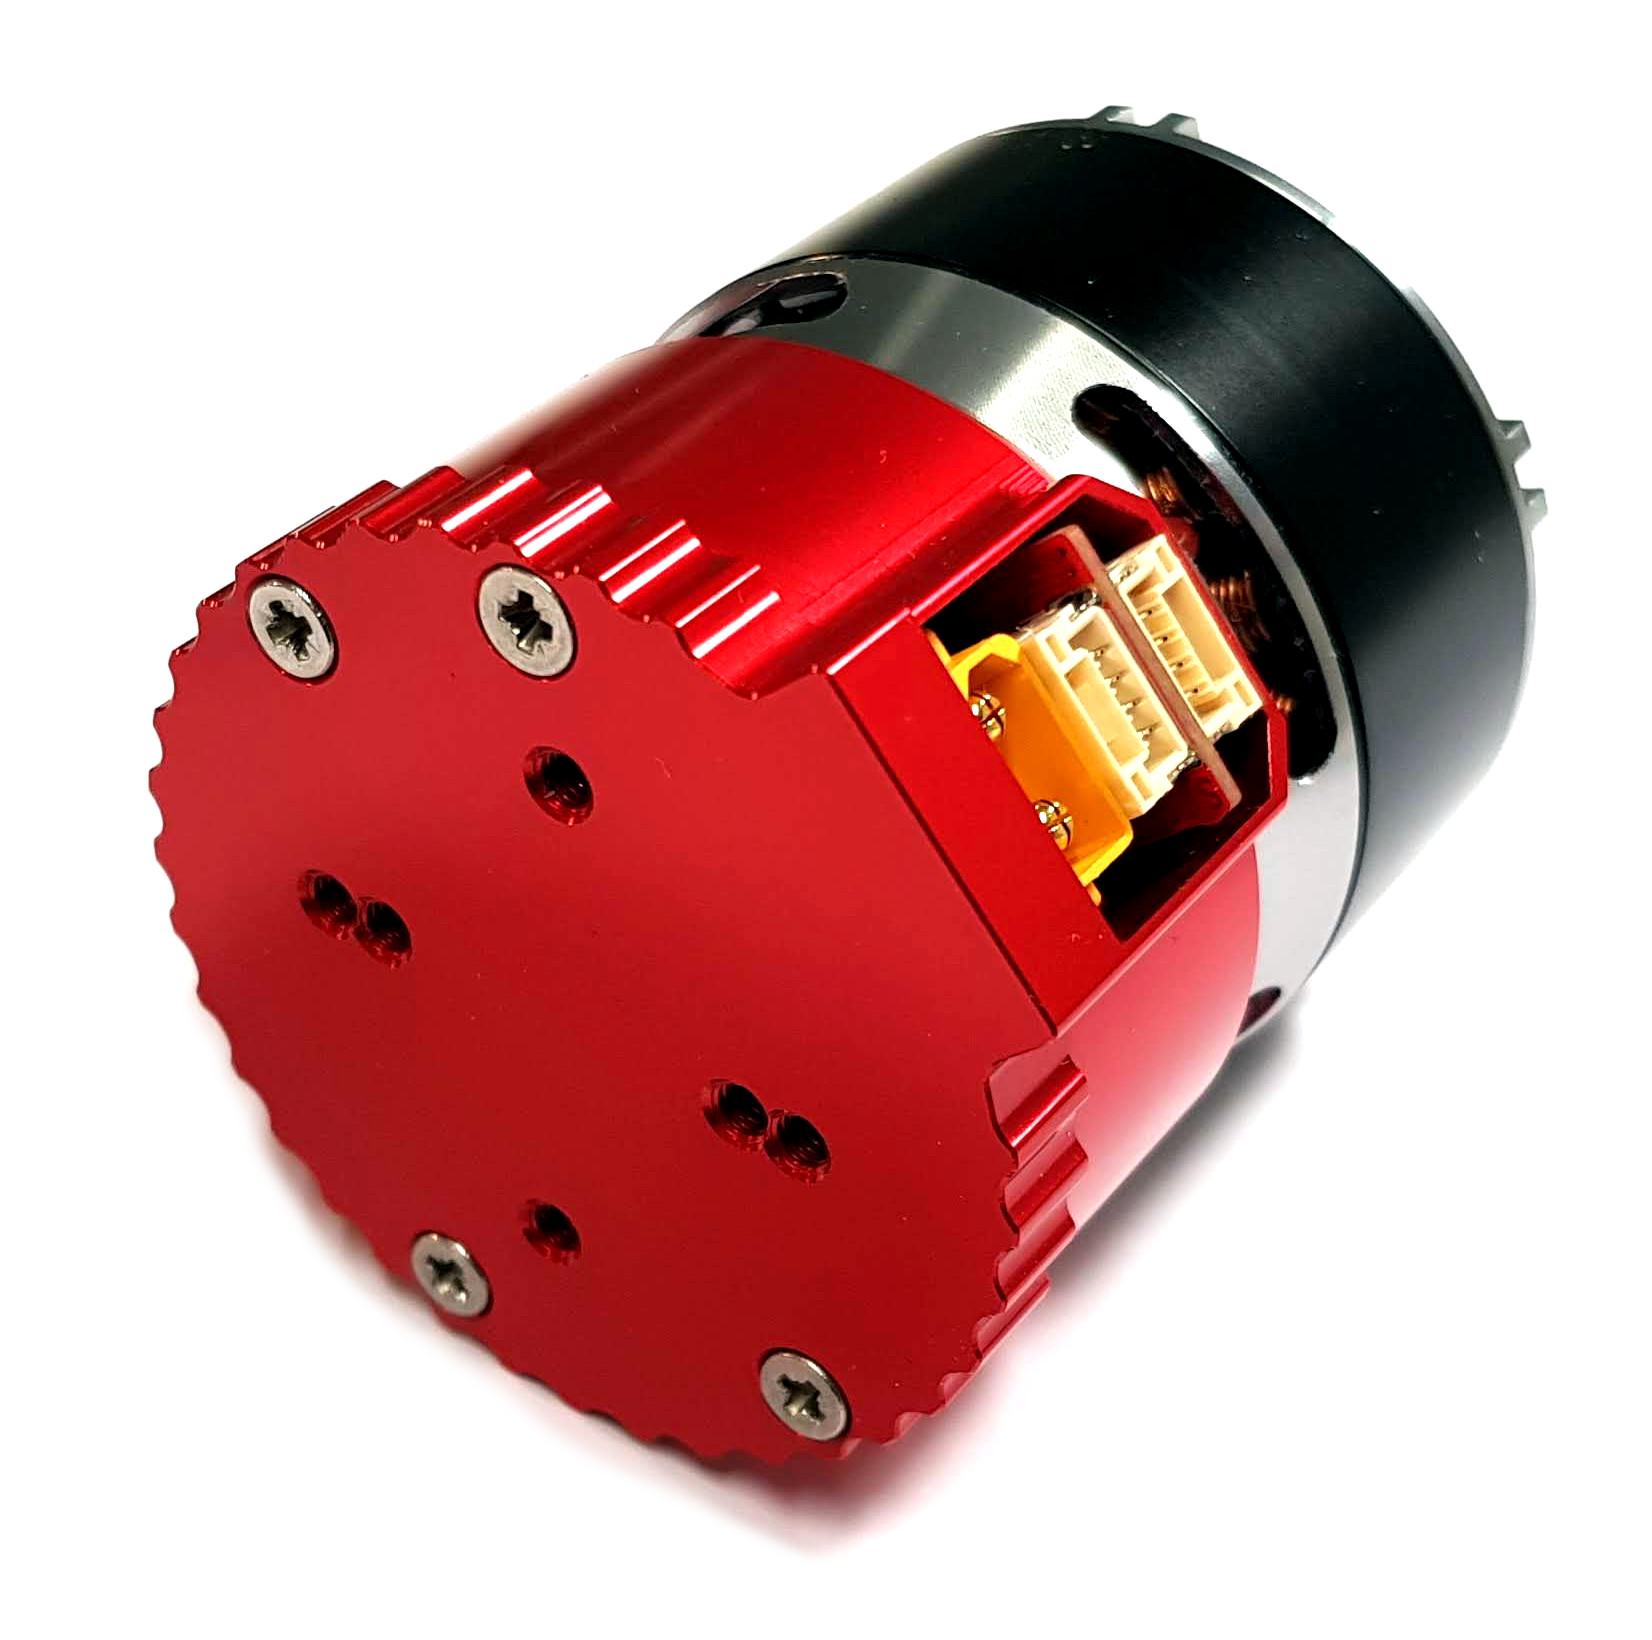
\includegraphics[width=0.42\textwidth]{sadulli-bottom}
\end{titlepage}

\tableofcontents
\BeginRightColumn
\listoffigures
\listoftables

\mainmatter

\chapter{Overview}

Zubax Sadulli is an open hardware reference design for Mitochondrik. It is a tightly integrated unit that contains 
an electric motor with sensorless electronic speed controller in a single monolithic package. 

Mitochondrik \footnote{Refer to \url{zubax.com/products/mitochondrik} for more information} is an integrated module 
(like an integrated circuit) that enables third-party hardware engineers to design sophisticated custom motor 
controllers using motor control technology -- Tele\-ga\footnote{Reefer to \url{zubax.com/technologies/telega} 
for more information}, which integrates advanced control algorithms. This datasheet is focused only on the Sadulli 
hardware.
  
The ESC is cooled by the motor. This allows for increasing the maximum ESC power in the same frame. 
Compact and tightly integrated design minimizes motor wiring and hence internal resistance. This, in turn, 
means fewer power losses and EMI. 

There are two versions of Sadulli: Sadulli Piccino and Sadulli Grosso. 
Sadulli Piccino can be applied for light multirotor aircraft with takeoff weight 500 - 800  g/rotor. 
While Sadulli Grosso can be applied for multirotor aircraft with takeoff weight 1300 g/rotor. 

\section{Quality assurance}

Every manufactured Zubax Mitochondrik undergoes an automated testing procedure that validates that
the device is functioning as designed.
The test log for every manufactured device is available on the web at
\url{https://device.zubax.com/device_info}.
This feature can be used to facilitate traceability of purchased devices and provide additional safety assurances.

Every manufactured device has a strong digital signature stored in its non-volatile memory
which proves the origins of the product and eliminates the risk of sourcing unlicensed or
counterfeit hardware.
This signature is referred to a Certificate of Authenticity (CoA).
Please refer to the section \ref{sec:certificate_of_authenticity} and visit the
\href{https://kb.zubax.com}{Zubax Knowledge Base} to learn more about
the certificate of authenticity and how it can be used to trace the origins of your hardware.


\section{Accessories}

Zubax Sadulli can be used with the following accessories:

\begin{itemize}
    \item 15x5 carbon fiber propeller for Sadulli Piccino (Figure \ref{1555 propeller}).
    \item 15x5.5 carbon fiber folding propeller for Sadulli Piccino (Figure \ref{1555 folding propeller}).
    \item 18x6.5 carbon propeller for Sadulli Grosso (Figure \ref{1865 propeller}). 
    \item 17x6.5 carbon fiber folding propeller for Sadulli Grosso (Figure \ref{1760 folding propeller}).    
    \item UAVCAN Micro patch cable.
    \item UAVCAN Micro termination plug.
    \item Power cable with XT30 connector
\end{itemize}

Please contact your supplier for ordering information.

\begin{figure}[tb]
    \centering
    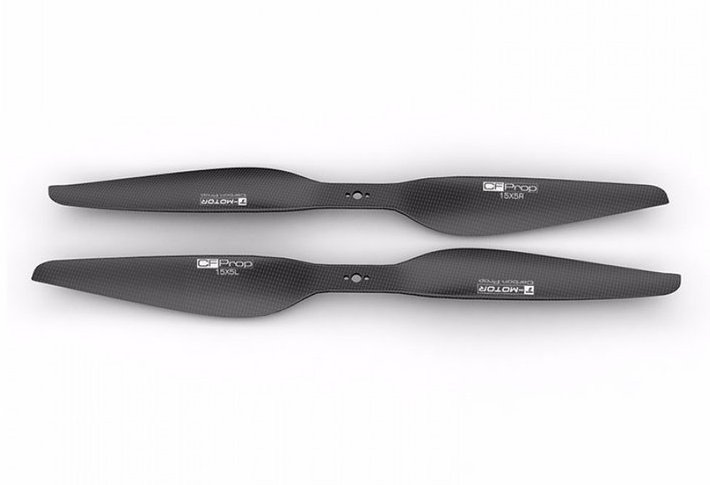
\includegraphics[width=0.45\textwidth]{1551propeller} 
    \caption{15x5 carbon fiber propeller.\label{1555 propeller}}
\end{figure}

\begin{figure}[tb]
    \centering
    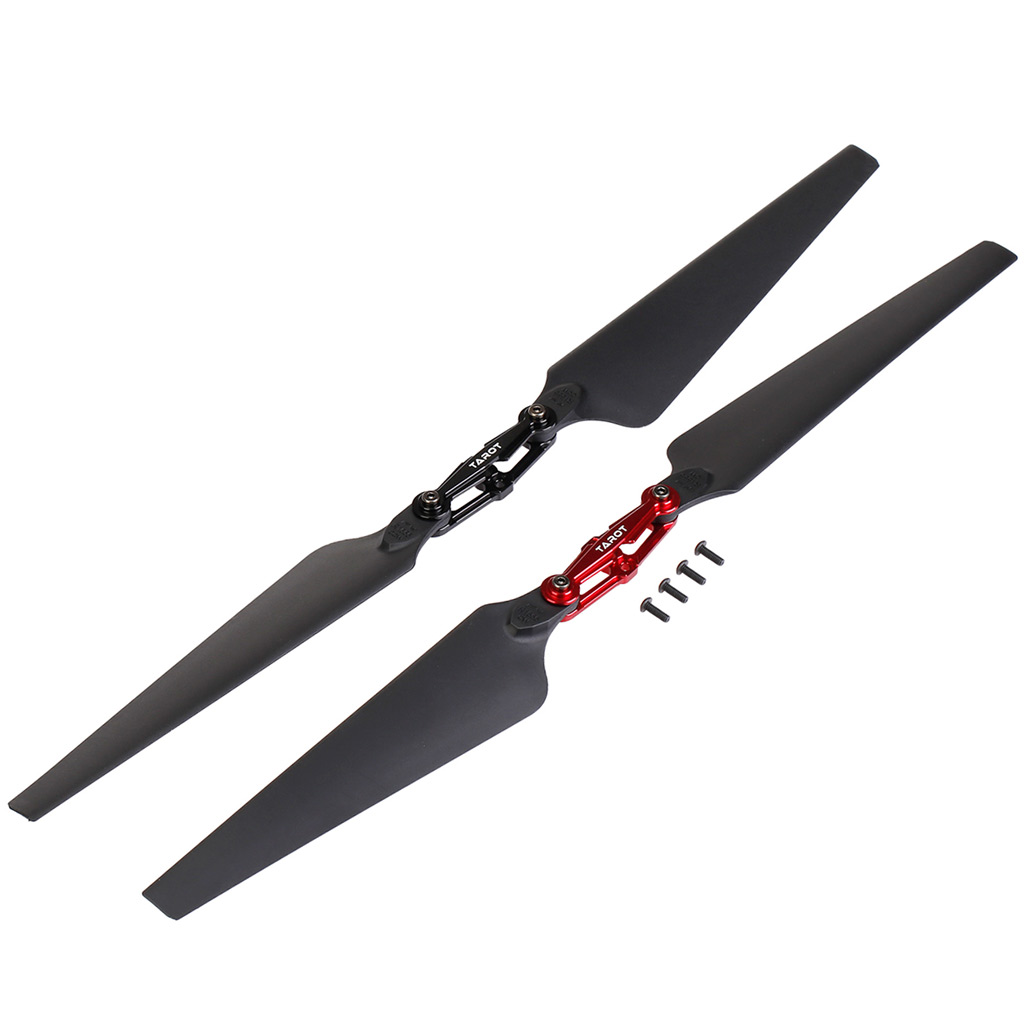
\includegraphics[width=0.45\textwidth]{1555propeller} 
    \caption{15x5.5 carbon fiber folding propeller.\label{1555 folding propeller}}
\end{figure}

\begin{figure}[tb]
    \centering
    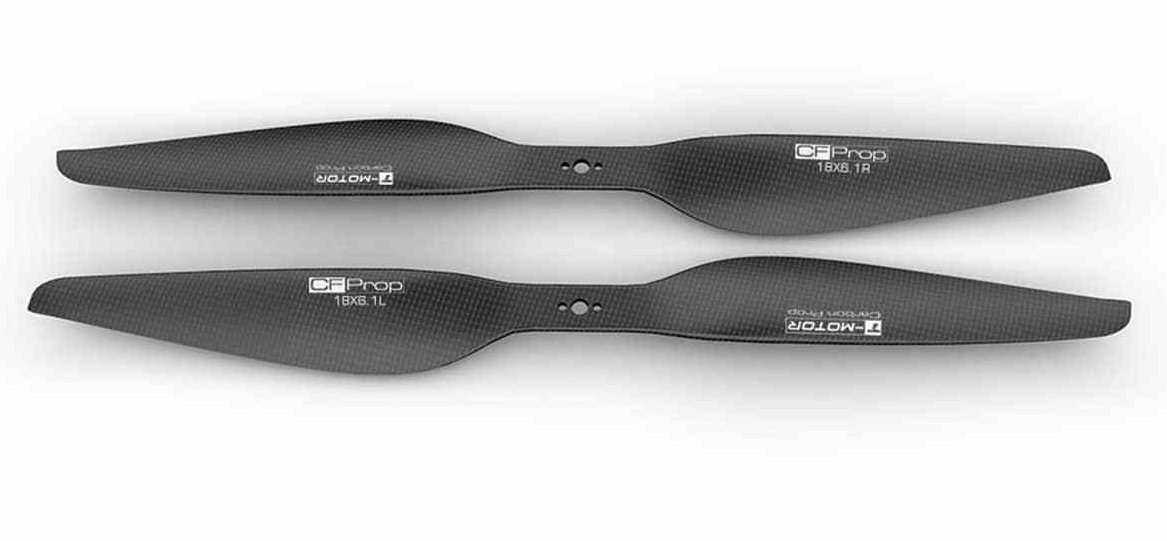
\includegraphics[width=0.45\textwidth]{1861propeller} 
    \caption{18x6.5 carbon fiber propeller.\label{1865 propeller}}
\end{figure}

\begin{figure}[tb]
    \centering
    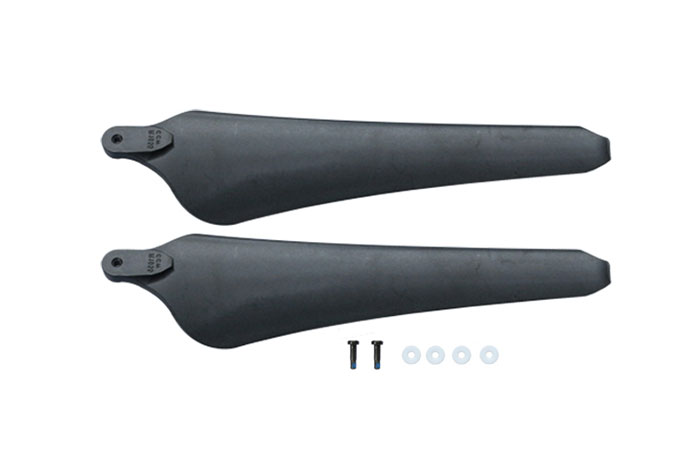
\includegraphics[width=0.45\textwidth]{1760propeller} 
    \caption{17x6.5 carbon fiber folding propeller.\label{1760 folding propeller}}
\end{figure}




\chapter{Characteristics}

\section{Absolute maximum ratings}

Stresses that exceed the limits specified in this section may cause permanent damage to the device.
Proper operation of the device within the limits specified in this section is not implied.

\begin{ZubaxSimpleTable}{Absolute maximum ratings}{|c X|c c|c|}
    Symbol            & Parameter                & Min  & Max & Unit \\
    $V_\text{inv}$    & Supply voltage           & -0.3 & 37  & V \\
    $T_\text{oper}$   & Operating temperature    & -50  & 125 & \degree{}C \\
                      & CAN H/L input voltage    & -4   & 16  & V\\
\end{ZubaxSimpleTable}

\section{Environmental conditions}

\begin{ZubaxSimpleTable}{Environmental conditions}{|c X|l|c c|c|}
    Symbol & Parameter & Note & Min & Max & Unit \\
    $T_\text{oper}$ & Operating temperature &                            & -40 & 105 & \degree{}C \\
    $T_\text{stor}$ & Storage temperature   &                            & -40 & 50  & \degree{}C \\
    $\phi_\text{oper}$ & Operating humidity & Condensation not permitted & 0   & 100 & \%RH\\
    $h_\text{oper}$ & Operating altitude    & Above mean sea level (MSL) &     & 10  & km\\
\end{ZubaxSimpleTable}

\section{Reliability}

Please contact Zubax Robotics for additional reliability and safety information.

\begin{ZubaxSimpleTable}{Reliability}{|c X|c|c|}
    Symbol & Parameter & Typ & Unit \\
    MTTF   & Mean time to failure & 20000 & hours \\
\end{ZubaxSimpleTable}

\section{Motor specification}

\begin{ZubaxSimpleTable}{Motor}{|c X|c|c|c|}
    Symbol & Parameter                                 & Sadulli Grosso & Sadulli Piccino & Unit \\
    N                    & Number of rotor poles       & 24             & 24              & - \\
    Kv                   & Constant velocity           & 330            & 380             & rpm/V \\
    $I_\text{noload}$    & No load current             & 0.7            & 0.3             & A/10V \\
    $I_\text{motor max}$ & Motor phase maximum current & 30             & 16              & A(30sec)\\
    $P_\text{motor max}$ & Motor maximum continious power & 750         & 450             & W \\
       -                 & Weight                       & 166           & 66              & g\\
\end{ZubaxSimpleTable}

\section{ESC characteristics}

\begin{ZubaxTableWrapper}{ESC characteristics}
    \begin{ZubaxWrappedTable}{|c X|c c c|c|}
        Symbol & Parameter & Min & Typ & Max & Unit \\
        $P$                 & Continuous power                    &      &      & 500  & W \\
        $P_\text{peak}$     & Peak power (30sec)                  &      &      & 600  & W \\
        $I_\text{inv}$      & Continuous DC current               &      &      & 20   & A \\
        $I_\text{inv-peak}$ & Peak DC current                     &      &      & 55   & A \\
        $I_\text{idle}$     & Idle current consumption            &      & 50   &      & mA \\
        $V_\text{inv}$      & Supply voltage\tnote{a}             & 12   &      & 36.0 & V \\
        $V_\text{TVS}$      & TVS\tnote{b}\space{} circuit
                              activation voltage                  & 37   &      & 40   & V \\
        $P_\text{TVS}$      & TVS circuit maximum power
                              dissipation                         &      & 1000 &      & W \\
        $E_\text{TVS}$      & TVS circuit energy absorption
                              capability\tnote{c}                 &      &  5   &      & J \\
        $R_\text{DS-on}$    & FET drain-source on-state resistance &      &  6  &   & $\text{m}\Omega$ \\
                            & Inverter temperature measurement
                              error                               & -6   &      & +6   & \degree{}C \\
                            & Inverter temperature measurement
                              range                               & -55  &      & 125  & \degree{}C \\
                            & Motor temperature measurement error & -8   &      & +8   & \degree{}C \\
                            & Motor temperature measurement
                              range                               & -50  &      & 175  & \degree{}C \\
                            & BEC output voltage                  &  4.8 & 5.0  & 5.1  & V \\
                            & BEC maximum output current          &      &      & 500  & mA \\
        
    \end{ZubaxWrappedTable}

\end{ZubaxTableWrapper}

\subsection{Power connectors}

Zubax Sadulli is equipped with XT30 battery power connector. 
The motor phases are connected internally direct to the power board. This minimizes motor wiring and 
hence internal resistance. 

\subsection{Motor temperature measurement}

Zubax Sadulli measures the temperature of motor windings by means of the KTY84/130 PTC thermistor. 
It converts and translates measured data via UAVCAN bus\footnote{Not all versions of Telega support 
motor temperature measurement. Refer for Telega documentation for more information}.  

\subsection{Regenerative braking}

During regenerative braking, the device performs energy transfer from the motor to the power supply network.
If the self-resistance of the power supply network is not sufficiently low,
the regenerative energy transfer may lead to an increase of the supply voltage beyond
the safe operating limits.
This event will trigger activation of the transient voltage suppression (TVS) circuit,
which will absorb some of the excessive energy.
If the amount of recovered energy exceeds the absorption capabilities of the power supply
network and the TVS circuit, the device may incur fatal damage.

Generally, batteries are capable of absorbing the energy recovered during braking without issues.
Problems may arise if the device is powered from a source that does not permit high reverse currents,
such as laboratory power supplies.
In that case, it is advised to install additional buffer capacitors to act as an energy storage
during braking.

\section{Communication interfaces}

\subsection{CAN bus}

The device is equipped with an ISO 11898-2 CAN 2.0A/B interface.
The CAN interface has two standard UAVCAN Micro connectors\footnote{Refer to \url{http://uavcan.org} 
for more information on UAVCAN.} joined in parallel. The power rails of the connector pair are connected via 
a switch to the device's BEC.

\begin{ZubaxSimpleTable}{CAN bus connectors pinout}{|c X X X[3]|}
    Pin no. & Type         & Name      & Comment \\
    1       & Power        & PWR       & Connected to the BEC via the switch.\\
    2       & Input/Output & CAN H     & \\
    3       & Input/Output & CAN L     & \\
    4       & Ground       & GND       & \\
\end{ZubaxSimpleTable}

\begin{ZubaxTableWrapper}{Characteristics of CAN bus interfaces}
    \begin{ZubaxWrappedTable}{|c X|c c c|c|}
        Symbol  & Parameter                                 & Min  & Typ  & Max  & Unit \\
                & Bit rate                                  & 20   &      & 1000 & Kbps \\
                & Positive-going input threshold voltage    &      & 750  & 900  & mV \\
                & Negative-going input threshold voltage    & 500  & 600  &      & mV \\
                & Differential output voltage, dominant     & 1.5  & 2.0  & 3.0  & V \\
                & Differential output voltage, recessive    & -120 & 0    & 12   & mV \\
                & Bus power rail\tnote{a}\space{} voltage   & -10  &      & 10   & V \\
                & Inter-connector current\tnote{a}          & -1 &  & 1    & A \\
                & Connector resistance during device lifetime &    & 30   & 50   & $\text{m}\Omega$ \\
    \end{ZubaxWrappedTable}
    \begin{tablenotes}
        \item [a] The limit is imposed by the PCB.
    \end{tablenotes}
\end{ZubaxTableWrapper}

\section{Indication}

Zubax Sadulli is equipped with a single RGB LED indicator for purposes of status indication and single Green LED for 
CAN bus transfer indication. These LEDs are located on the PCB near the UAVCAN connectors.

\section{Mechanical characteristics}

The drawings \ref{Sadulli_grosso_drawing} and \ref{Sadulli_piccino_drawing} document the basic mechanical 
characteristics of Zubax Sadulli, such as dimensions and propeller mounting holes placement.

Sadulli is mounting on the chassis like a motor. It has standard  19x25 and 25x25 mounting patterns. These patterns are
shown on the drawing \ref{Sadulli_mounting_drawing}).

\begin{figure}[tb]
    \centering    
    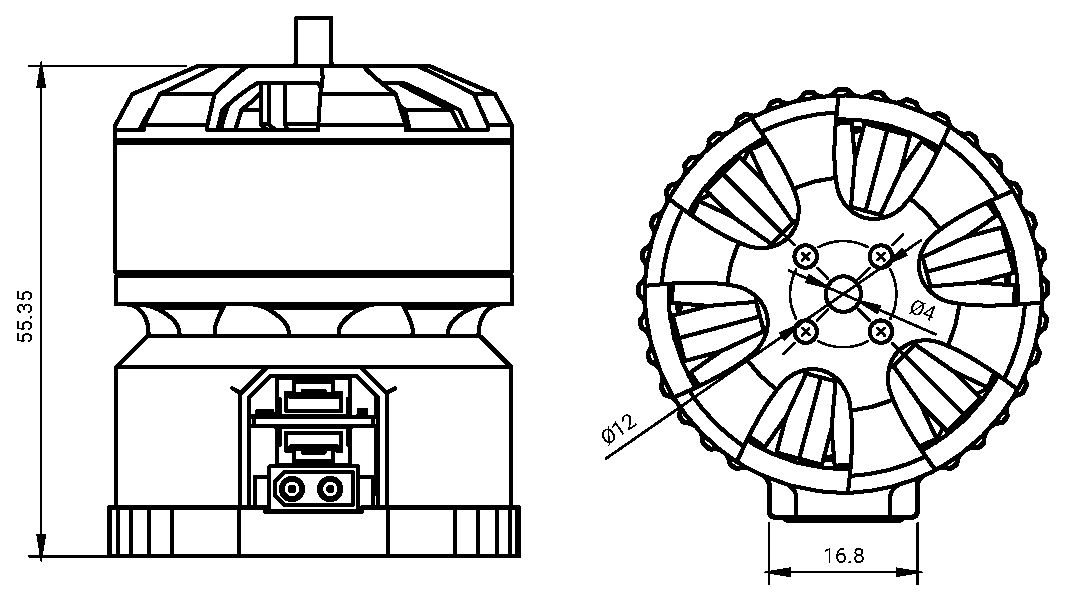
\includegraphics[width=0.65\textwidth]{sadulli-grosso_drawing}
    \caption{Sadulli-grosso drawing.\label{Sadulli_grosso_drawing}} 
\end{figure}

\begin{figure}[b]
    \centering    
    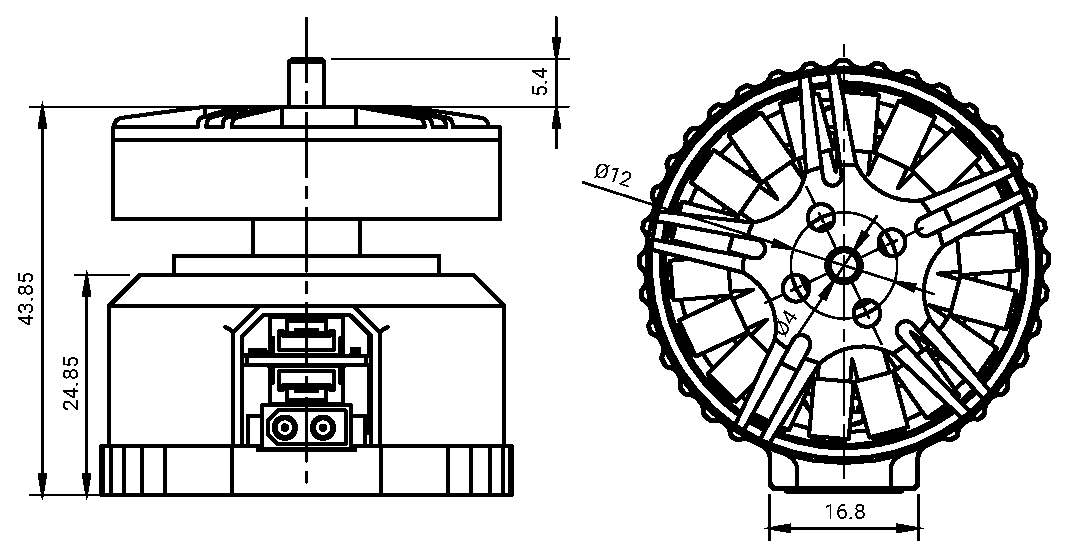
\includegraphics[width=0.65\textwidth]{sadulli-piccino_drawing}
    \caption{Sadulli-piccino drawing.\label{Sadulli_piccino_drawing}}
\end{figure}

\begin{figure}[b]
    \centering    
    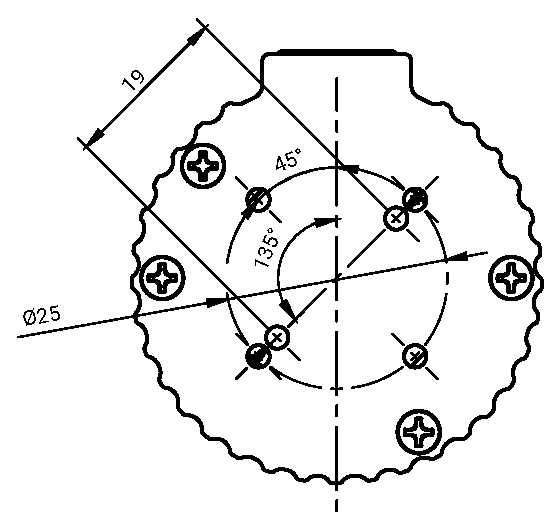
\includegraphics[width=0.45\textwidth]{mounting_drawing}
    \caption{Sadulli mounting drawing.\label{Sadulli_mounting_drawing}}
\end{figure}


\begin{ZubaxSimpleTable}{Mechanical characteristics}{|c|l|c|c|с|X|}
    Symbol & Parameter   & Grosso  &Piccino  & Unit & Note                 \\
    $m$    & Weight      & 207     & 128     & g    & Cables not included  \\
    IP     & Ptotection  & 65      & 65      & -    & The ESC is conformally coated to protect 
                                                      from wet conditions \\                        
\end{ZubaxSimpleTable}

\chapter{Operation}\label{operation}
\section{System connection}\label{sec:system_connection}

No soldering is required to connect Zubax Sadulli to the application system. 
It is ready to use right out of the box. Just plug in battery XT30 power connector and CAN interface 
(RCPWM optionally) UAVCAN microconnectors as shown in Figure \ref{Sadulli_connectors}. 

The BEC can be activated in the firmware and is applied to the power rails of the UAVCAN connectors.
Application-specific integration documentation is available on the Zubax Knowledge Base at
\mbox{\url{https://kb.zubax.com} and \url{https://zubax.com/technologies/telega}}

\begin{figure}[hb]
    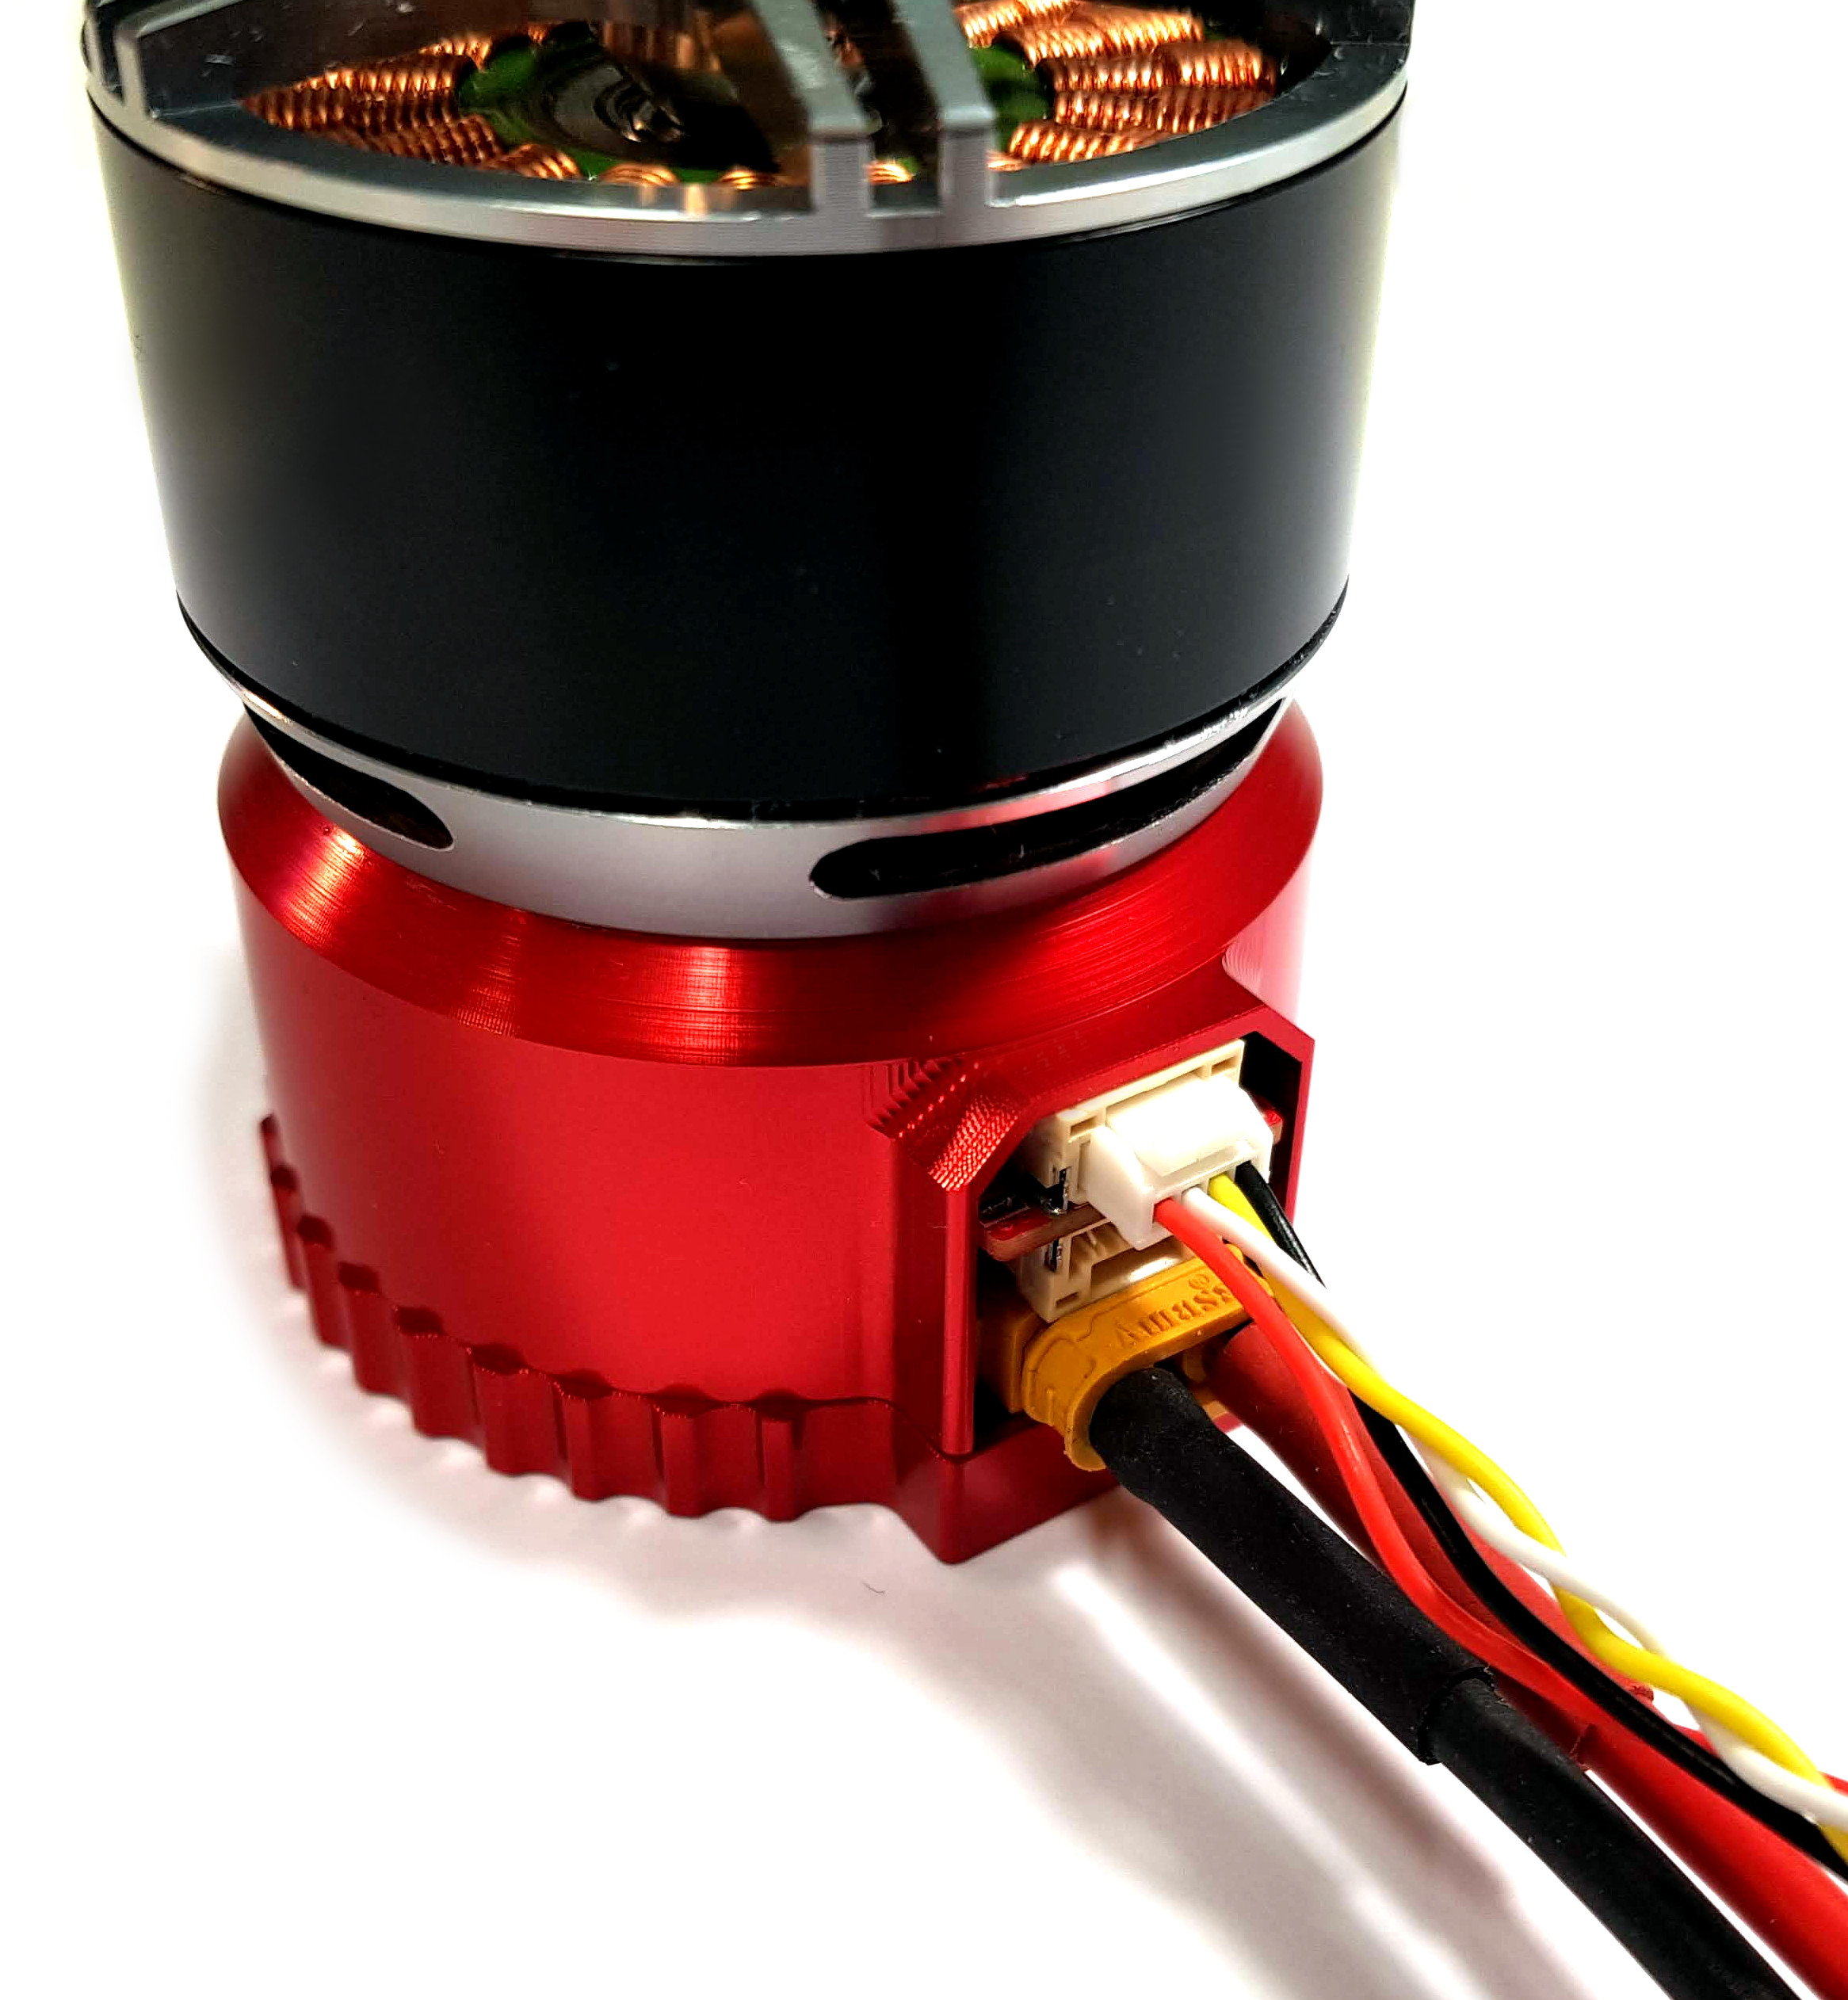
\includegraphics[width=0.45\textwidth]{sadulli-connectors} 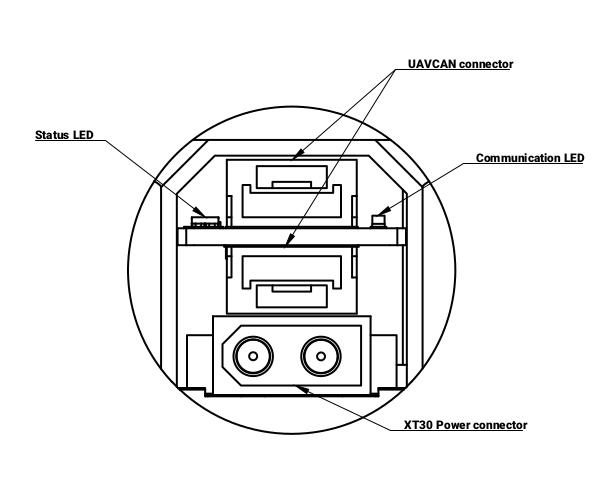
\includegraphics[width=0.45\textwidth]{connectors}
    \caption{Connection of Sadulli.\label{Sadulli_connectors}}
\end{figure}


\section{LED indicators}

\newcommand{\LEDX}{{\rule{0.4em}{1.0em}}}
\newcommand{\LEDO}{{\rule{0.4em}{0.1em}}}

\newcommand{\ShowColor}[1]{{\color{#1}\rule{2em}{0.8em}}}

Zubax Sadulli is equipped with two separate LED indicators that reflect the current state of the device.

The green traffic LED indicates data transfer through the CAN bus. Blinks once if at least one CAN frame 
was successfully transmitted or successfully received in the last 25~milliseconds. Glows steadily when 
the intensity of CAN traffic is higher than 40 frames per second.

The behavior of the RGB status LED is more complex than the traffic LED. 
It is specified in the tables \ref{table:status_led} and \ref{table:status_led_behavior}.

\begin{ZubaxSimpleTable}{Status LED during boot}{|l l X|}\label{table:status_led}
    Color                     & Status                          & Description \\
    \ShowColor{yellow} Yellow & No application to boot          & The firmware haven't been flashed to the ESC
                                                                  or FLASH has been damaged. \\
    \ShowColor{blue} Blue     & Application upgrade is in progress. &            \\
    \ShowColor{green} Green   & Boot canceled                   & The device firmware has not been properly signed \\
    \ShowColor{magenta} Magenta & Ready to boot                 & Glows after power up or restart the device until 
    the application starts\\
\end{ZubaxSimpleTable}

\begin{ZubaxSimpleTable}{Status LED behavior}{|l X X|}\label{table:status_led_behavior}
    LED pattern (step 80 ms) & Status & Description\\

    {\color{blue}
       \LEDX\LEDO\LEDO\LEDO\LEDO\LEDX} & Idle, ready to run & The ESC is ready and waiting for the setpoint\\
    
    {\color{red}
       \LEDX\LEDO\LEDO\LEDO\LEDO\LEDX\LEDX\LEDX} & Idle, Hardware fault & The power stage is not ready or current is 
       tripped\\

    {\color{red}
       \LEDX\LEDO\LEDO\LEDO\LEDO\LEDX\LEDO\LEDX\LEDX\LEDX} & Idle, Hardware test fault & The motor is not connected or 
       there is a short circuit on the output of the ESC\\

    {\color{red}
       \LEDX\LEDO\LEDO\LEDO\LEDO\LEDX\LEDO\LEDX\LEDO\LEDX\LEDO\LEDX\LEDO\LEDX\LEDO\LEDX\LEDO\LEDX\LEDX\LEDX\LEDO\LEDX
       \LEDX\LEDX} & Idle, Invalid motor parameters & Some motor parameters are not properly initialized or the motor 
       identification hasn't been performed\\

\end{ZubaxSimpleTable}

\section{Device identification}

\subsection{Hardware version number}

Zubax Sadulli reports to the Telega firmware the following hardware version number
(in the form major.minor): 1.7. It actually is the Mitochondrik hardware version number because Sadulli is based on 
the Mitochondrik module. 

\subsection{Certificate of authenticity}\label{sec:certificate_of_authenticity}

The Telega firmware can report the certificate of authenticity (CoA),
if one is found installed on the hardware that the firmware is running on.
The details covering how to request the CoA from Telega fall outside of the scope of this document;
the reader is advised to refer to the Telega Reference Manual for explanations.

Every manufactured instance of Zubax Mitochondrik contains a valid CoA, which is an RSA-1024 digital signature
\end{document}
